\section{Introducción}
\noindent La espectroscopia es el estudio de la interacción entre la radiación electromagnética y la materia, con absorción o emisión de energía radiante. En la primera parte de la práctica tendremos como finalidad medir la absorbancia de ambas muestras mediante un espectrofotómetro. El dispositivo que vamos a usar nos dará directamente la absorbancia, aunque también se puede calcular con:

\[A = \epsilon\cdot{l}\cdot{c}\]

\vspace{0.2cm}

\noindent donde $A$ será la absorbancia, $\epsilon$ el coeficiente de absorción molar, $l$ la longitud (= 1cm) y $c$ la concentración.

\noindent Aunque por la ley de Lambert Beer, la absorción vendrá dada por: $A = -log(T)$

\vspace{0.1cm}

%%%%%%%%VEEERRR

\noindent En la segunda parte formaremos moléculas de los principales grupos y las nombraremos.

\section{Inventario}
\noindent En esta práctica contamos con:

\begin{multicols}{2}
    \begin{itemize}
        \item 4 tubos de ensayo
        \item 3 vasos de precipitados
        \item Un espectrofotómetro
        \item Un matraz aforado
        \item Azul bromotimol
        \item Remazol
        \item Blanco (\ce{H2SO4})
        \item Una propipeta
        \item Una pipeta graduada
    \end{itemize}
\end{multicols}

\begin{figure}[H]
    \centering
    \hspace*{-2.3cm}
        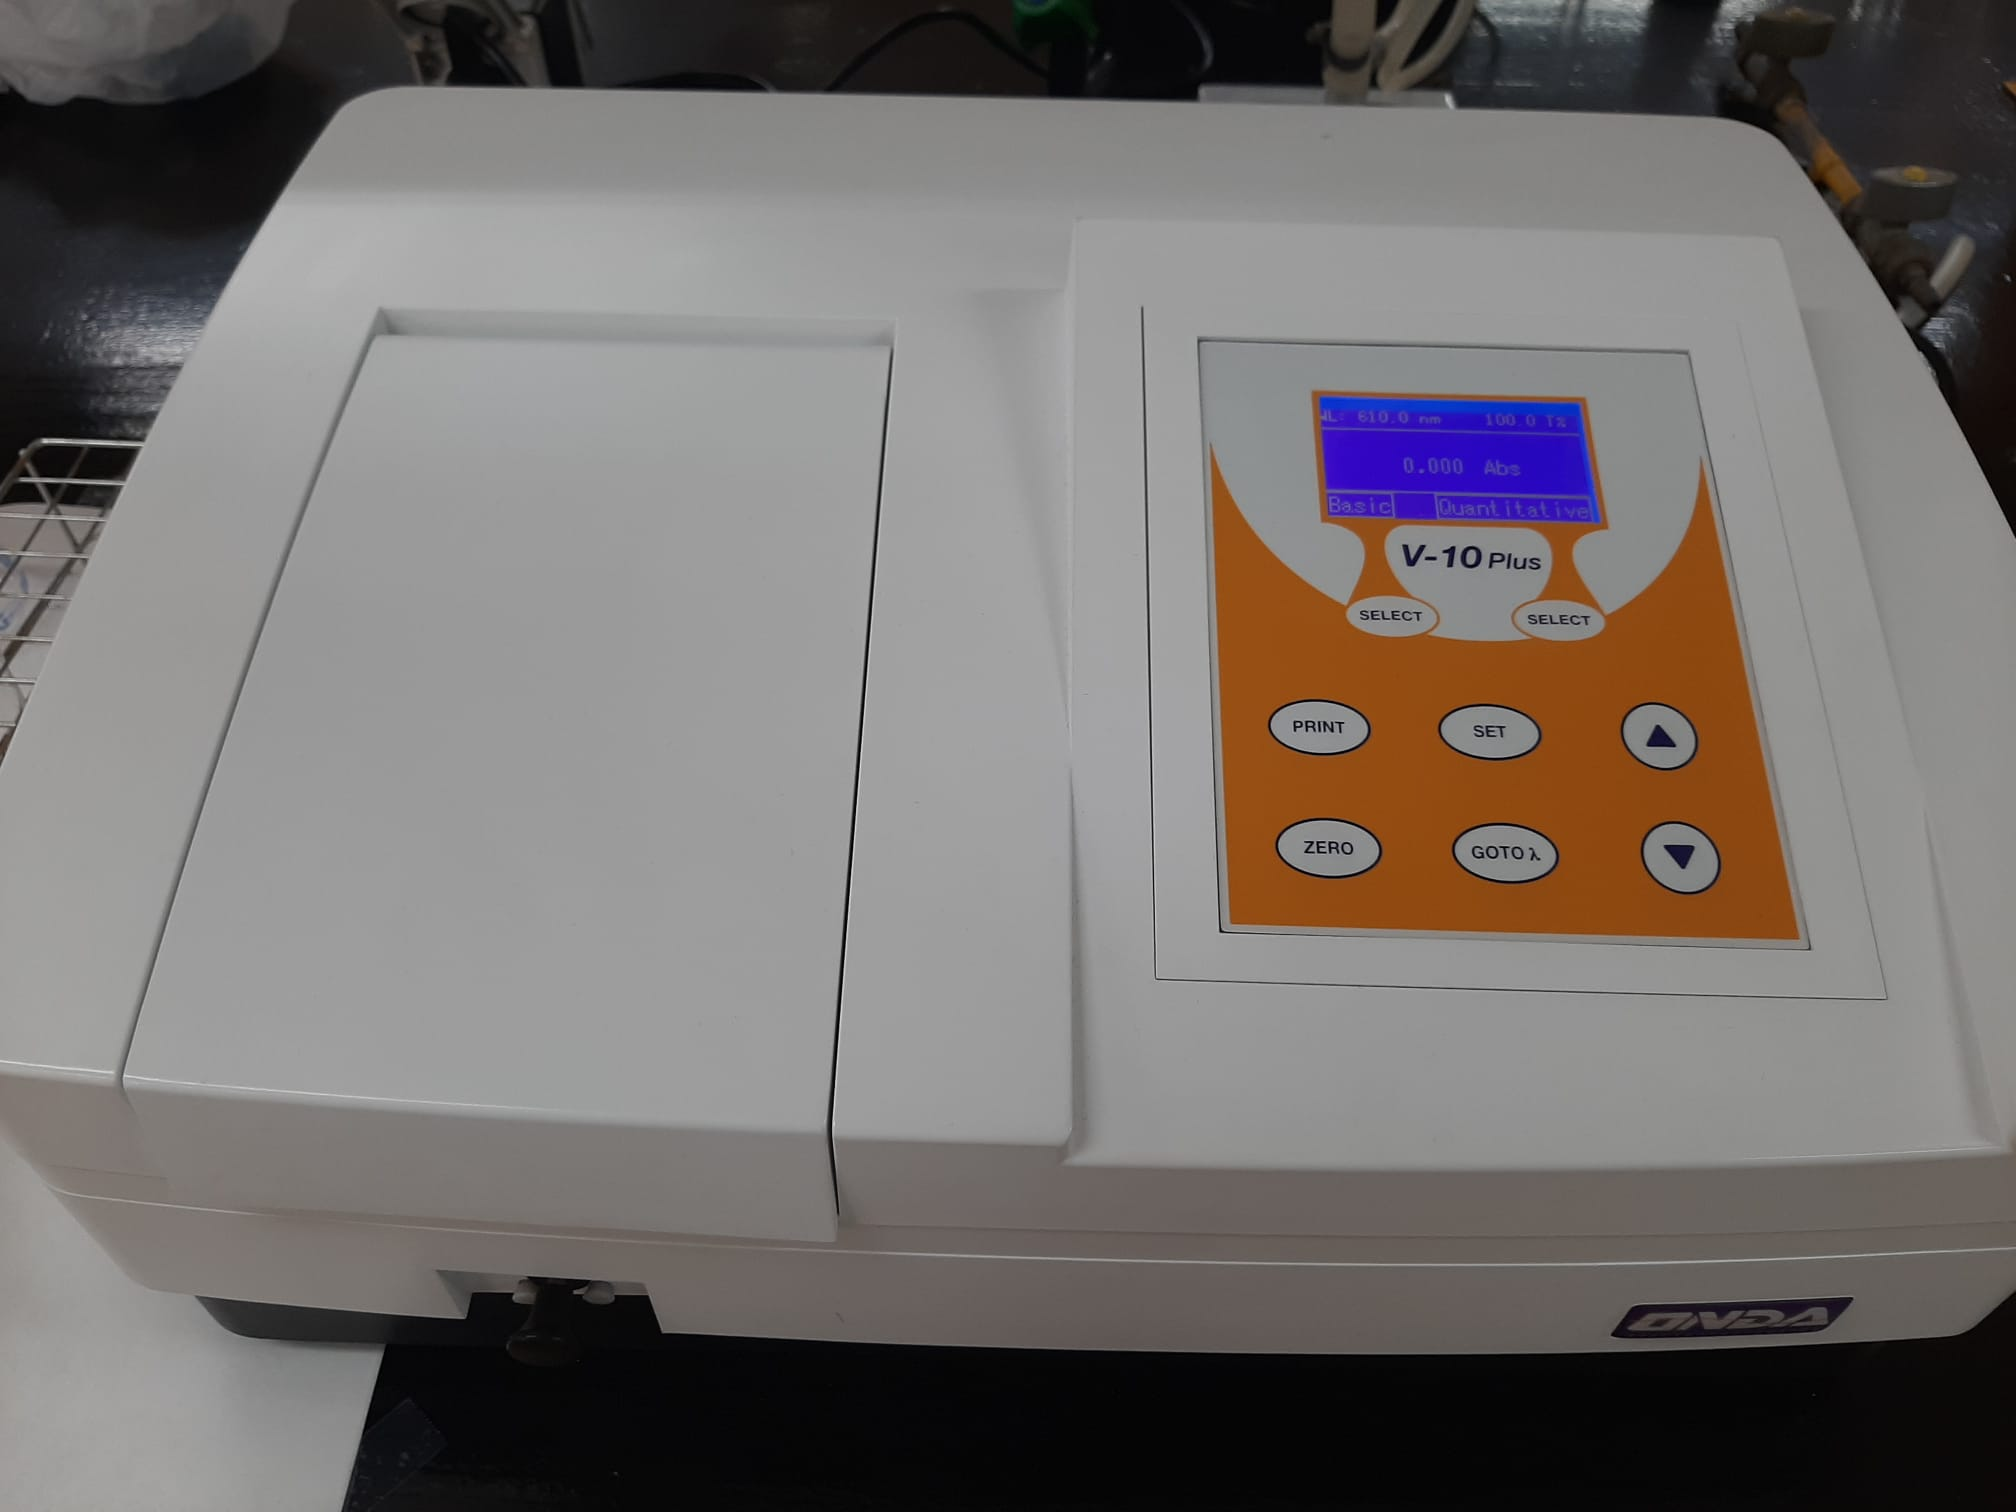
\includegraphics[scale = 0.07]{fotos/instru.jpeg}
        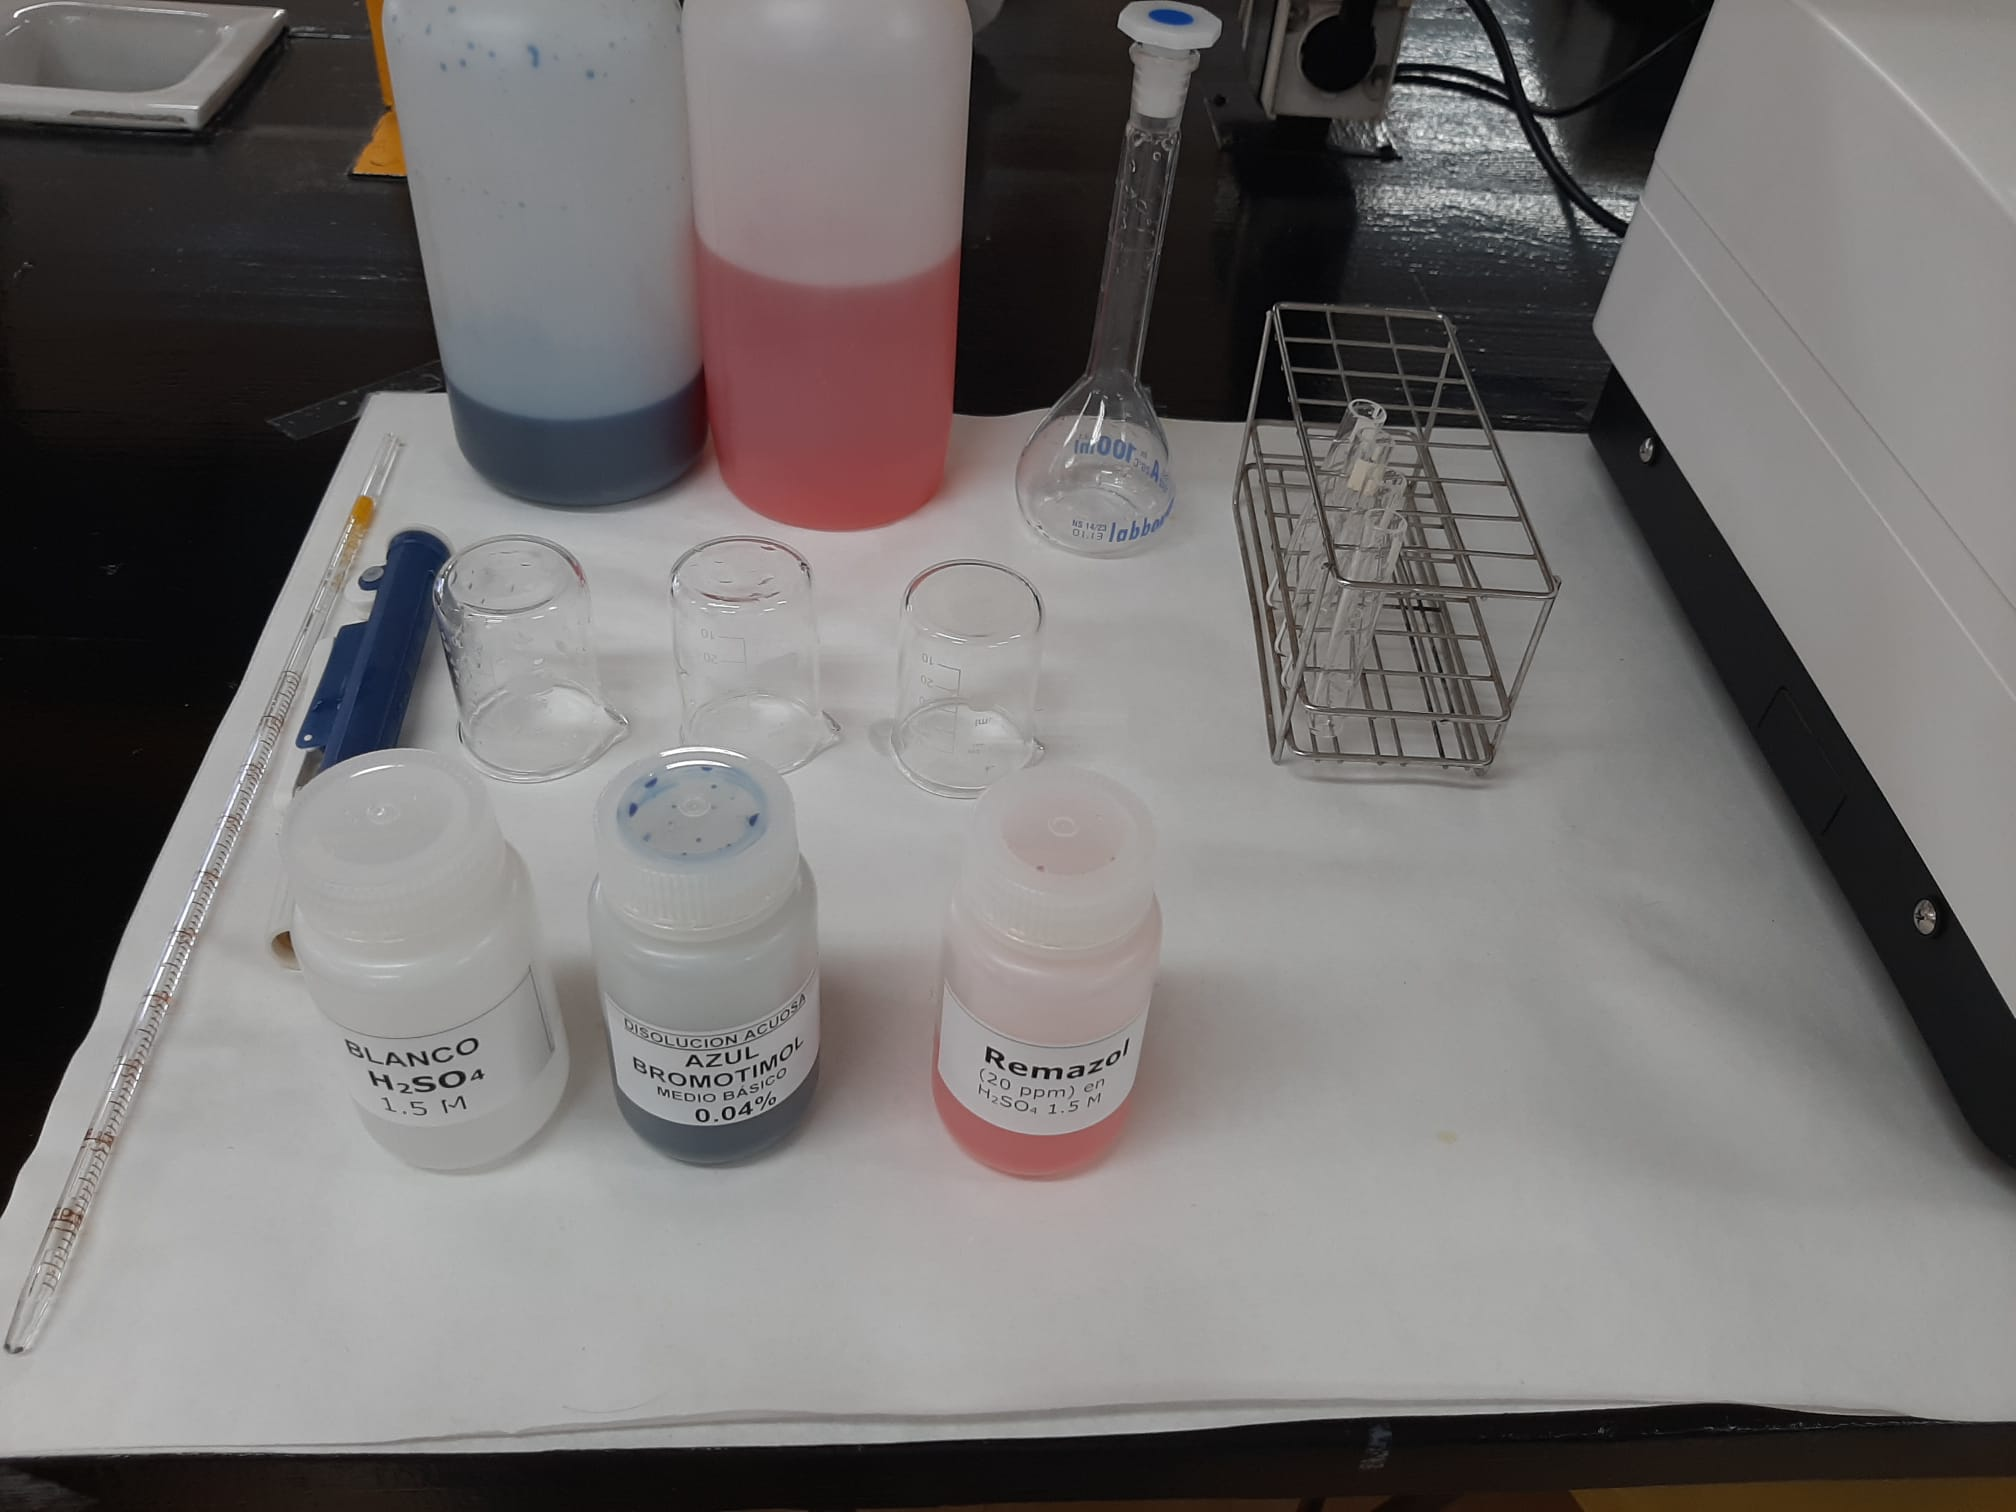
\includegraphics[scale = 0.07]{fotos/set8.jpeg}
    \hspace*{-2.3cm}
    \caption{Material utilizado, a la izquierda el espectrofotómetro y a la derecha el material usado}
\end{figure}
\clearpage

\section{Procedimiento}
\noindent En primer lugar, empezaremos la práctica preparando en cuatro cubetas, una con agua destilada, otra con azul bromotimol, otra con remazol y por último una con blanco(\ce{H2SO4}). Una vez hecho esto, nos dispondremos a empezar la práctica, teniendo que medir la absorbancia de cada muestra para determinadas longitudes de onda. Para ello, deberemos ajustar convenientemente la absorbancia del blanco a 0, y ya podremos medir la de la muestra.\\

%\vspace{0.2cm}

\noindent Cabe destacar que en la práctica había dos instrumentos distintos, uno más moderno y otro más antiguo. En nuestro caso, tuvimos el privilegio de contar con el nuevo, ya que nos permitía poner el blanco y nuestra muestra junta, sin necesidad de evaluar a cada longitud de onda el blanco y sacarlo para poner la muestra; es decir, nosotros colocábamos ambas cubetas y sólo debíamos tirar de una especie de barra metálica, a continuación dejo una foto para que sea más gráfico.

\vspace{0.4cm}

\begin{figure}[H]
    \centering
    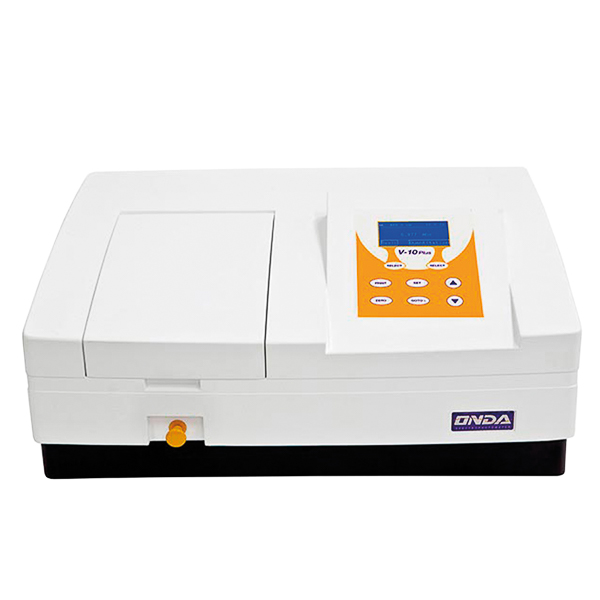
\includegraphics[scale = 0.2]{fotos/SPTR-V01-001.jpg}
    \caption{Espectrofotómetro visible, ONDA V-10 PLUS}
    \label{fig:cris}
\end{figure}

\vspace{0.4cm}


\noindent Primeramente, hacemos una dilución del Azul de bromotimol en un matraz aforado, con $1 mL$ de azul y $99 mL$ de agua (hasta llegar al máximo) y le agregamos una gota de de \ce{NaOH} $0.1M$.\\

\noindent Usaremos como blanco agua destilada y como muestra la disolución previamente explicada.\\

\noindent Una vez puestos los dos tubos de ensayo en el espectofotómetro, anotaremos la absorbancia para la diferentes longitudes de onda. Lo evaluaremos en el rango de 450 hasta 700 nanometros, aumentando la longitud de onda a razón de $10 nm$, y nos anotaremos en qué punto el valor de la absorbancia será mayor. Luego haremos una segunda pasada, donde abarcaremos un rango de -10nm y +10nm tomando como referencia el punto donde la absorbancia es mayor y mediremos dicho valor cambiando la longitud de onda de 2 en 2, para obtener así un resultado más preciso.\\


\noindent Una vez terminado lo anterior, cambiaremos los tubos de ensayo por blanco(\ce{H2SO4}) y la muestra de remazol. Haremos lo mismo que en el paso previo, solo que ahora el rango de la longitud de onda va de 400 a 600 nm. \\

\noindent Los datos obtenidos así como la gráfica de los datos lo veremos en el apartado de las cuestiones.



\vspace{0.6cm}
%%%%%%VEEEEEEEEERRR PTEE 2




\noindent \textit{2. Mediante el uso de modelos moleculares construya las moléculas de azul de bromotimol y remazol RB 133, e identifique los principales grupos funcionales y
estructuras orgánicas sencillas.}\\

\noindent Principales grupos funcionales: cada uno de los tres anillos aromáticos compone, junto a los grupos metilos y tertbutilo, el grupo timol, el nombre 'bromotimol'msurge de tener enlazado un Br.\\

\noindent A continuación, expongo unas fotografías de los distintos grupos y estructuras orgánicas que hemos reproducido en el laboratorio:


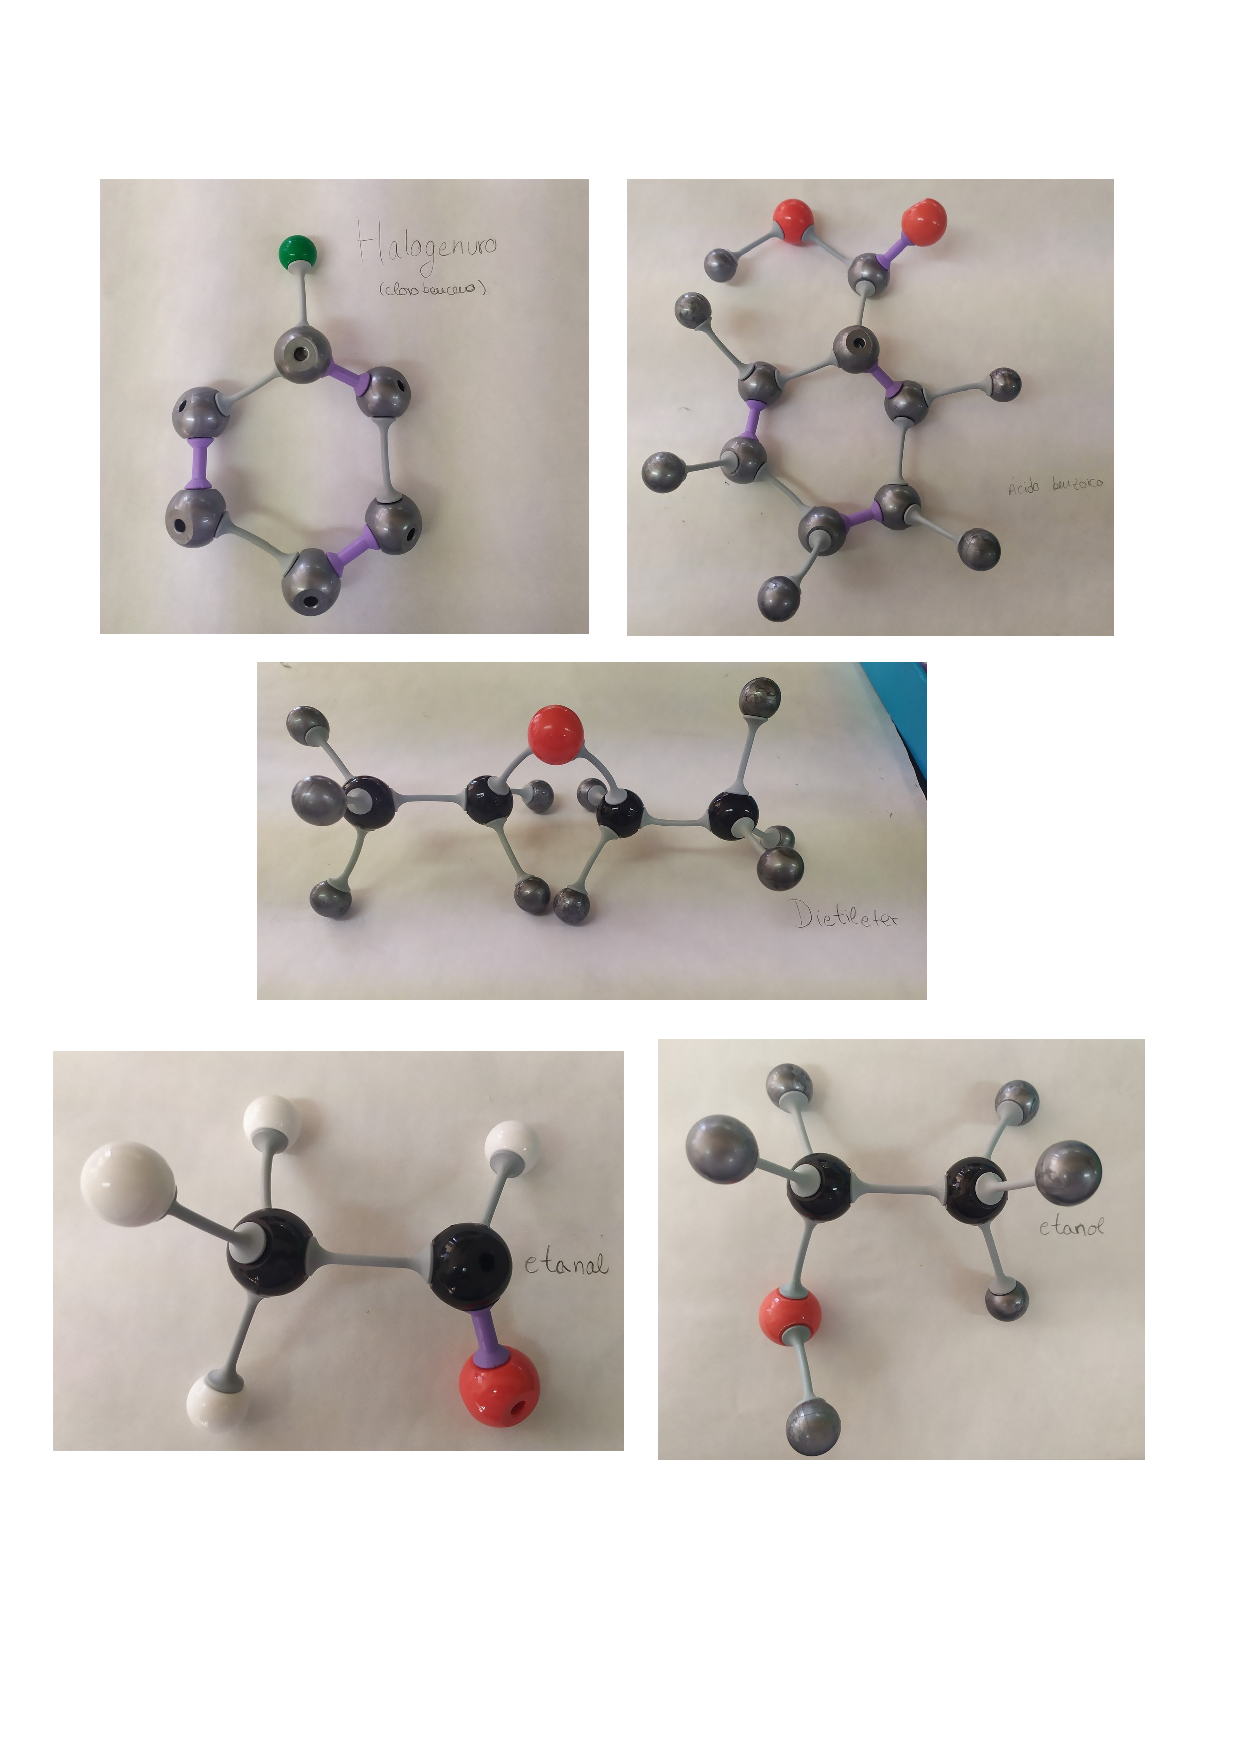
\includepdf[pages=-]{fotitos.pdf}



\clearpage

\section{Cuestiones}

\noindent\textcolor{BlueViolet}{\textbf{\textit{a) Determine el coeficiente de absorción molar del azul de bromotimol. Compare, si es posible, el resultado con el reportado en la bibliografía.}}}


\noindent El coeficiente de absorción puede expresarse por:

\[\epsilon = \frac{A}{l \cdot c}\]
 
\noindent siendo c la concentración, y la absorción la hemos calculado tal como hemos explicado en el procedimiento.

\vspace{0.4cm}

\begin{figure}[H]
    \centering
    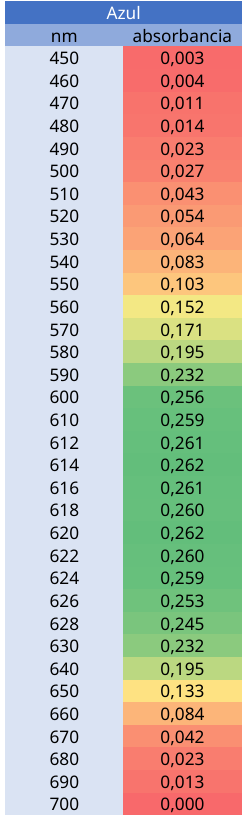
\includegraphics[scale = 0.333]{fotos/tabla azul.png}    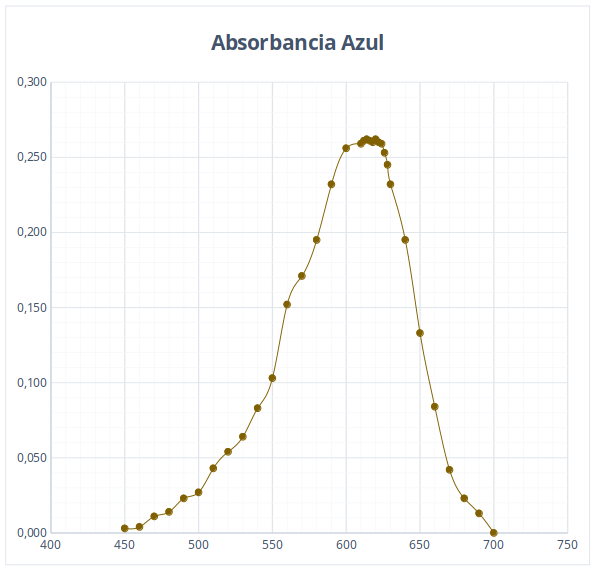
\includegraphics[scale = 0.433]{fotos/abs azul.png}
    \caption{Medidas tomadas y la correspondiente gráfica}
    \label{fig:cris}
\end{figure}

\vspace{0.4cm}

\noindent En la tabla, el color verde nos indica que hemos alcanzado el pico y por ello medimos para longitudes de onda que difieren de dos nanometros.

\noindent En esta gráfica podemos observar como $\epsilon$ varía con la longitud de onda de la luz, siendo este el gráfico del espectro de absorción. \\

\noindent A partir de estos datos, tomando el máximo valor de la gráfica podemos calcular el coeficiente de absorción mediante $A = \epsilon\cdot{l}\cdot{[concentración]}$, despejando tenemos que $\epsilon = \frac{0.262}{0.01\cdot{1.3}\cdot 10^{-4}}$ = \underline{$2.02\cdot{10^{5}}$}\\


\clearpage

\noindent\textcolor{BlueViolet}{\textbf{\textit{b) Determine el coeficiente de absorción molar del remazol RB 133. Compare, si es
posible, el resultado con el reportado en la bibliografía.}}}\\


\noindent Este apartado es similar al anterior, pero en lugar de tratar con azul de bromotimol usamos remazol RB 133.\\

\vspace{0.4cm}

\begin{figure}[H]
    \centering
    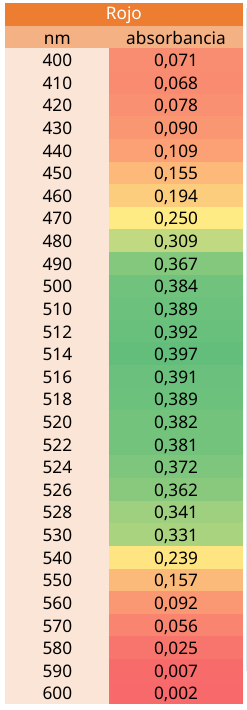
\includegraphics[scale = 0.333]{fotos/tabla rojo.png} 
    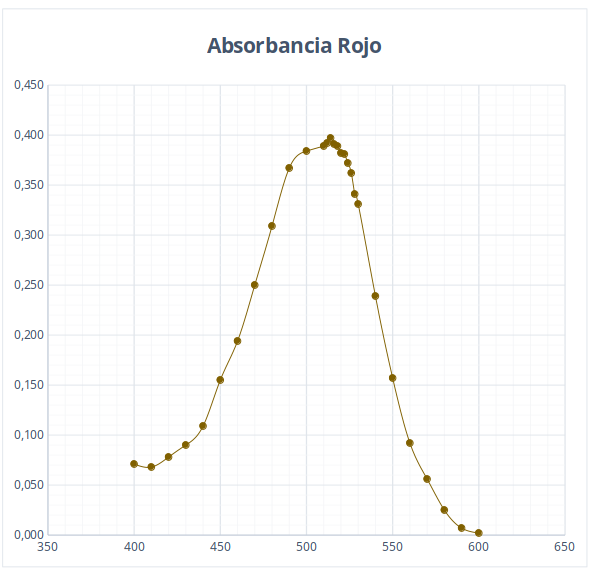
\includegraphics[scale = 0.433]{fotos/abs rojo.png}   
    \caption{Medidas tomadas y la correspondiente gráfica}
    \label{fig:cris}
\end{figure}

\vspace{0.4cm}

\noindent En esta gráfica podemos observar como la variación de la absorbancia en función de la longitud de onda de la luz, siendo este el gráfico del espectro de absorción, al igual que hemos visto en \textit{a)}. Además, a modo de aclaración, el color verde nos indica que hemos alcanzado el pico y es por eso que pasamos a medir la absorción para longitudes de onda que difieren en dos nanometros.\\


\noindent A partir de estos datos, tomando el máximo valor de la gráfica podemos calcular el coeficiente de absorción mediante $A = \epsilon\cdot{l}\cdot{[azul de bromotimol]}$, despejando tenemos que $\epsilon = \frac{0.397}{0.01\cdot{1}\cdot 10^{-4}}$ = \underline{$2.26\cdot{10^{5}}$}\\

\noindent No es posible comparar el resultado con el reportado en la bibliografía ya que no está, igual que para el apartado anterior. 


\clearpage

\noindent\textcolor{BlueViolet}{\textbf{\textit{c) Del apartado 2 del procedimiento, nombre las moléculas orgánicas de acuerdo con la nomenclatura de química orgánica.}}}\\


\noindent A continuación desarrollo una tabla en la que se encuentran formulados los compuestos de los que hay imágenes en la parte dos de la práctica:\\

\begin{table}[H]
\centering
\begin{tabular}{|l|c|}
\hline
\textbf{Nombre}                   & \textbf{Fórmula} \\ \hline
Halogenuro: clorobenceno          &         $C_6H_5Cl$            \\ \hline
Éter: dietiléter                  &         $(C_2H_5)_2O$         \\ \hline
Alcohol: etanol                   &         $C_2H_5OH$         \\ \hline
Aldehído: etanal                  &         $C_2H_4O$         \\ \hline
Ácido carboxílico: ácido benzoico &         $C_7H_6O_2$         \\ \hline
Éster: acetato de etilo           &         $C_4H_8O_2$     \\ \hline
Amida primaria: propanamida       &         $C_3H_7NO$         \\ \hline
Ácido salicílico                  &         $C_7H_6O_3$         \\ \hline
Ácido acetilsalicílico            &         $C_9H_8O_4$         \\ \hline
Naftaleno                         &         $C_{10}H_8$         \\ \hline
Ciclohexano                       &         $C_6H_{12}$         \\ \hline
Ciclopropano                      &         $C_3H_6$         \\ \hline
Ciclobutano                       &         $C_4H_8$         \\ \hline
Etano                             &         $C_2H_6$         \\ \hline
Eteno                             &         $C_2H_4$         \\ \hline
Etino                             &         $C_2H_2$         \\ \hline
Tiofeno                           &         $C_4H_4S$         \\ \hline
Sulfóxido de tiofeno              &         $C_4H_4SO$         \\ \hline
Sulfona de tiofeno                &         $C_4H_4SO_2$         \\ \hline
\end{tabular}
\end{table}

\vspace{0.3cm}

\noindent En esta tabla podemos diferenciar 4 grupos: del halogenuro al naftaleno pertenecen al \textbf{benceno y sus derivados}; los ciclo- pertenecen a los \textbf{compuestos cíclicos}; el etano, etano y etino a los \textbf{hidrocarburos} y los tres últimos pertenecen al \textbf{tiofeno y derivados}. Podemos observar que estos elementos son los que hemos puesto las fotografías en el apartado del desarrollo.








